Related work for this project is divided among three fields: algorithms for ACL injury detection (Section 2.1), knee brace effectiveness/performance hindrance (Section 2.2), and Knee Mechanical Properties (Section 2.3).

\subsection{ACL Injury Detection} This section covers research in minimizing the testing required to detect whether an athlete is at risk of suffering an ACL injury. Prior research in ACL Injury Detection has shown that techniques exist that accurately capture and analyze various measures relating to the knee to determine the probability of ACL injuries \cite{smedicine}. Using such metrics as knee flexion angles, medial rotation, and body mass, researchers were able to come up with a way to determine knee abduction moments (KAM), which are used to identify whether or not an athlete is at high risk for an ACL injury, with a sensitivity of 77\% and specificity of 71\% \cite{smedicine}\cite{Bahr01062005}. 

\subsection{Knee Brace Effectiveness/ Performance Hindrance} This section deals mainly with studies of the extent to which a Functional Knee Brace and a Prophylactic Knee Brace interacts with an athlete's ability to perform on the field. Prior research in using Functional or Prophylactic knee braces out in the field has shown that it potentially hinders an athlete's movement by restricting the anterior translation. In addition, the studies on the usefulness of these kinds of braces in preventing the injury are inconclusive \cite{Myer01042011}. Knee braces, especially Functional Knee Braces (FKB), which are more mechanical in nature and thus more obtrusive, are shown to provide \"20-30\% greater knee ligament protection\". This suggests that while FKBs have an impact in reducing the severity of knee injuries, there is an opportunity to come up with a new brace to evaluate the risk index and thereby provide proof for the capability of existing braces. Another important factor of the effectiveness of knee braces is in rehabilitation, where a combination of exercises and brace use can speed up recovery \cite{hewett2010acl}. eKwip can also provide evidence for establishing the usefulness of these exercises.

\subsection{Knee Mechanical Properties} Research has proved that the relative angle and forces between the femur and tibia are a major risk indicator to ACL injury. The paper \textsl{Shin, et al. 2006} provides the numerical data, which we will use to calculate the risk index for the athlete. As shown in Figure~\ref{fig:flex_angles} and Figure~\ref{fig:quad_force}, the authors of the paper created a model to track the knee flexion angle and the forces over time and found correlation with the experimental model of the injury. \cite{Shin20071145}


\begin{figure}[h]
  \begin{center}
    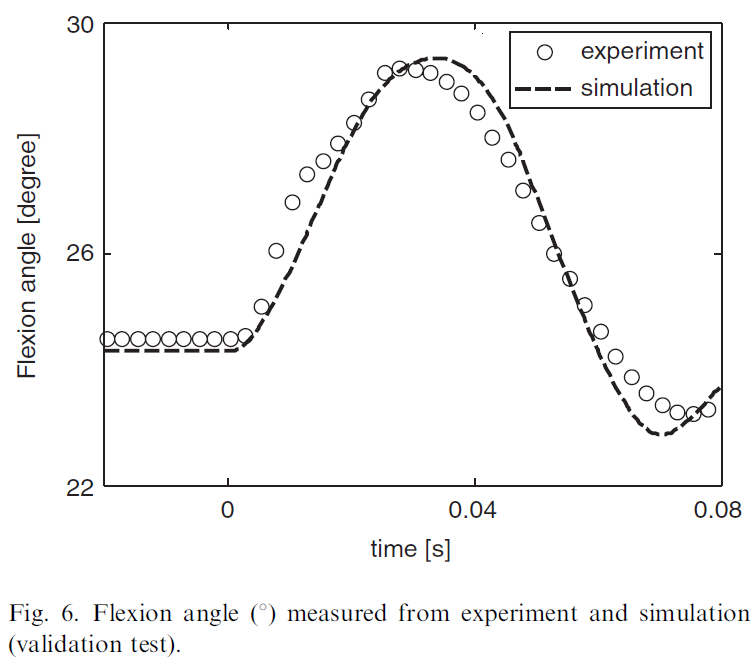
\includegraphics[width=3in]{images/flexangle.PNG}
  \end{center}
  \caption{Knee flexion angle over time during an ACL injury}
  \label{fig:flex_angles}
\end{figure}

\begin{figure}[h]
  \begin{center}
    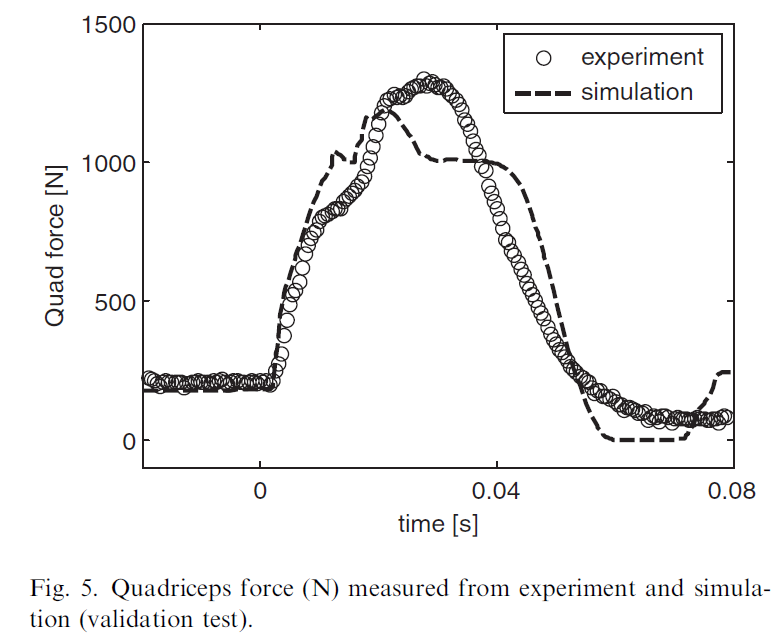
\includegraphics[width=3in]{images/quadforce.PNG}
  \end{center}
  \caption{Quad forces over time during an ACL injury}
  \label{fig:quad_force}
\end{figure}
